
\documentclass[11pt,a4paper]{article}
\usepackage[hyperref]{naaclhlt2019}
\usepackage{times}
\usepackage{latexsym}
\usepackage{graphicx}
\usepackage[normalem]{ulem}

\usepackage[utf8]{inputenc} % allow utf-8 input
\usepackage[T1]{fontenc}    % use 8-bit T1 fonts
\usepackage{hyperref}       % hyperlinks
\usepackage{url}            % simple URL typesetting
\usepackage{booktabs}       % professional-quality tables
\usepackage{amsfonts}       % blackboard math symbols
\usepackage{nicefrac}       % compact symbols for 1/2, etc.
\usepackage{microtype}      % microtypography
\usepackage{indentfirst}
\usepackage{soul}

\usepackage{url}

\aclfinalcopy 


\title{Analysis of RNN-Attention Machine Translation Methods}

\author{Stephen Dong  \\
  {\tt stdong@ucsd.edu} \\}
  % Second Author \\
  % {\tt email@domain} \\\And
  % Third Author \\
  % {\tt email@domain} \\\And
  % Fourth Author \\
  % {\tt email@domain} \\}
  
% \setlength\textwidth{16.0cm}
\date{}

\begin{document}
\maketitle

% \begin{abstract}
% \end{abstract}

 
% \section{Instructions}
%   {\color{blue}
%  \begin{itemize}
%      \item \textit{Length: Should be at least \textbf{5 pages} but not more than 8 pages. {Do not include this template content in your final report as it messes up page count}. 
%       Comment out everything in this document (except the headings when necessary)}
          
%      \item \textit{Submit (report, and optional code):  on Gradescope by \textbf{Friday, June 7, 2024}.}
%  \end{itemize} 
%  }

\section{Introduction}
% Original before both GPT proofread (this also includes any personal changes to information that might've been included after proofreaing that was not passed into GPT)
% This survey paper will focus on the analysis of neural machine translation (NMT). Machine Translation (MT) is a powerful automation tool to bridge the gap between languages by providing end-to-end translation between two languages. Translation tools like Google Translate have been an integral part of our society for the past few decades. Early MT tools have primarily been utilized to translate words and eventually simple phrases, but were still relatively inaccurate with more complex linguistics and sentences \cite{WANG2022143}. 

% Early MT approaches relied on rule-based methods; however, these approaches were tedious as they required manual translation from a dictionary. The 1990s saw the initial proposal of corpus-based statistical machine translation (SMT) models. Phrase-based SMT methods were later introduced in 2003 with "Pharaoh" and "Moses" as the primary innovations. \cite{WANG2022143} 

% Simple SMTs remained the dominant implementation of MT models until Nal Kalchbrenner, et al. \cite{kalchbrenner-blunsom-2013-recurrent} proposed the first NMT model that used an encoder-decoder structure for end-to-end translation. The paper proposed the recurrent continuous translation model (RCTM), which uses a convolutional neural network (CNN) in the encoder and an inverted CNN followed by a recurrent neural network (RNN) for the decoder. 

% Following this proposal, KyungHyun Cho et al. reveals a seperate alternative approach similar to Kalchbrenner's RCTM model that also incorporates the RNN into the encoder \cite{cho2014learning}. The paper also proposed a variation of the long-short term memory (LSTM) hidden unit, later denoted as a gated recurrent unit (GRU), to solve issues with retaining distant relevant information in longer sentences, allowing for higher BLEU scores as shown in Figure 1.

% The proposed GRU contains two primary gates: reset and update, shown in Figure 2. The update gate controls what new information from the new hidden state should be included in the hidden state. Meanwhile, the reset gate drops any information that displays signs of irrelevancy. These gates allow the unit to mimic long-term and short-term memory, i.e. long-term memory has more update gate activations and short-term memory with reset gates activations. \cite{cho2014learning} These gates allow the GRU to capture information in more meaningfully ways to boost performance.

% The models presented in both papers served as the backbone of future NMT models. The following years introduced the use of attention in MT models, with Google pushing out their state-of-the-art GNMT model for Google Translate \cite{wu2016googles}. The same year, Dzmitry Bahdanau et al. published their paper Neural Machine Translation By Jointly Learning to Align and Translate \cite{bahdanau2016neural}, which adds an attention mechanism to the GRU encoder-decoder model proposed by Cho.

% This survey will explore the attention-based RNN encoder-decoder model presented by Bahdanau et al. \cite{bahdanau2016neural}. This approach adds an attention mechanism in the decoder and converts the uni-directional encoder into a bi-directional RNN to extract and retain information behind and in front of each token. The paper suggests the model is capable of achieving an increased BLEU score of any long sentence translations.

% This paper will demonstrate the continued limitations of the attention RNN encoder-decoder model with longer and more complex sentence structures. This is an important consideration as recent increases in tourism around the world have prompted the need for accurate translations of large passages all at once. The codebase used for this survey is a smaller scaled tutorial implementation of the PyTorch seq2seq module \cite{github}. This codebase was also chosen for its accurate reflection of the model presented by the paper, but scaled down for hardware limitations. Results presented in this survey will be analyzed with this consideration. The results of the test set of the original codebase's dataset for both the attention and attention-less RNN encoder-decoder model will serve as the baselines.

% After GPT Proofread
This survey paper will focus on the analysis of neural machine translation (NMT). Machine Translation (MT) is a powerful automation tool to bridge the gap between languages by providing end-to-end translation between two languages. Translation tools like Google Translate have been an integral part of our society for the past few decades. Early MT tools primarily translated words and eventually simple phrases but were still relatively inaccurate with more complex linguistics and sentences \cite{WANG2022143}.

Early MT approaches relied on rule-based methods; however, these approaches were tedious as they required manual translation from a dictionary. The 1990s saw the initial proposal of corpus-based statistical machine translation (SMT) models. Phrase-based SMT methods were later introduced in 2003 with "Pharaoh" and "Moses" as the primary innovations, but these could only accurately translate smaller phrases. \cite{WANG2022143}

SMTs remained the dominant implementation of MT models until Nal Kalchbrenner, et al. \cite{kalchbrenner-blunsom-2013-recurrent} proposed the an NMT model that used an encoder-decoder structure for end-to-end translation. The paper proposed the recurrent continuous translation model (RCTM), which uses a convolutional neural network (CNN) in the encoder and an inverted CNN followed by a recurrent neural network (RNN) for the decoder.

Following this proposal, KyungHyun Cho et al. revealed a separate alternative approach similar to Kalchbrenner's RCTM model that also incorporates the RNN into the encoder \cite{cho2014learning}. The paper also proposed a variation of the long-short term memory (LSTM) hidden unit, later denoted as a gated recurrent unit (GRU), to solve issues with retaining distant relevant information in longer sentences, allowing for higher BLEU scores as shown in Figure 1.

\begin{figure}[h]
    \centering
    % \includegraphics[width=0.475\linewidth]{figures/LM_Default_Dropout/LM_Loss_Dropout.png}
    % \includegraphics[width=0.475\linewidth]{figures/LM_Default_Dropout/LM_Per_Dropout.png}
    \begin{tabular}{| l || c |}
    \hline
    Model & BLEU Test\\
    \hline
    \hline
    RCTM I + WP & 21.5\\
    RCTM II + WP & 21.7\\
    \hline
    RNN & 33.87\\
    CSLM + RNN & 34.64\\
    CSLM + RNN + WP & 34.54\\
    \hline
    \end{tabular}
    \caption{Side-by-side BLEU test results comparison of RCTMs \cite{kalchbrenner-blunsom-2013-recurrent} with word penalty (WP) and RNN and LSTM based encoder-decoder and semantic retention models with and without WP \cite{cho2014learning}}
\end{figure}

The proposed GRU contains two primary gates: reset and update, shown in Figure 2. The update gate controls what new information from the new hidden state should be included in the hidden state. Meanwhile, the reset gate drops any information that displays signs of irrelevancy. These gates allow the unit to mimic long-term and short-term memory, i.e. long-term memory has more update gate activations and short-term memory with reset gates activations. \cite{cho2014learning} These gates allow the GRU to capture information in more meaningfully ways to boost performance.

\begin{figure}[h]
    \centering
    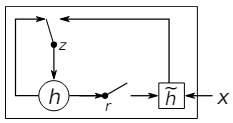
\includegraphics[]{figs/GRU_hidden_cell.png}
    \caption{GRU illustration from Cho et al.'s paper \cite{cho2014learning} with $z$ as the update gate, $r$ as the reset gate, $h$ as the current hidden state, and $\widetilde{h}$ as the new hidden state with new $x$ information.} 
\end{figure}

The models presented in both papers served as the backbone of future NMT models. The following years introduced the use of attention in MT models, with Google pushing out their state-of-the-art GNMT model for Google Translate \cite{wu2016googles}. The same year, Dzmitry Bahdanau et al. published their paper \textit{Neural Machine Translation By Jointly Learning to Align and Translate} \cite{bahdanau2016neural}, which adds an attention mechanism to the GRU encoder-decoder model proposed by Cho.

This survey will explore the attention-based RNN encoder-decoder model presented by Bahdanau et al. \cite{bahdanau2016neural}. This approach adds an attention mechanism in the decoder and converts the unidirectional encoder into a bidirectional RNN to extract and retain information behind and in front of each token. The paper suggests the model is capable of achieving an increased BLEU score of any long sentence translations. 

This paper will demonstrate the continued limitations of the attention RNN encoder-decoder model with longer and more complex sentence structures. This is an important consideration as recent increases in tourism around the world have prompted the need for accurate translations of large passages all at once. The codebase used for this survey is a smaller scaled tutorial implementation of the PyTorch seq2seq module \cite{github}. This codebase was also chosen for its accurate reflection of the model presented by the paper, but scaled down for hardware limitations. Results presented in this survey will be analyzed with this consideration. The BLEU scores of the test set of the original codebase's dataset for both the attention and attention-less RNN encoder-decoder model will serve as baselines.

% \textbf{Task and Model Summary}: Briefly summarize the NLP \textbf{problem or task} chosen and explain its importance. Specify the \textbf{model or system} selected, including references to the paper and the source code. (It is fine if  your task is different from the one in your proposal.)

% \noindent \textbf{Approach and Findings Summary}: Describe the approach taken for analyzing the system. Summarize the main limitations identified during the analysis.


\section{The Dataset and Model}
\subsection{Training}
The original dataset \cite{elliott-EtAl:2016:VL16} provided by the codebase is used to train a model for German-English translations. The dataset contains a much smaller set of approximately 32K sentence translations of approximately 400K words compared to the approximately 348M words of the original paper \cite{bahdanau2016neural}. 20,518,405 parameters are learnable during training and is validated on 1,014 en-de translations. 1,000 en-de translations are used to test the capabilities of the model. All preprocessing and model implementations will be the default provided by the codebase.

This dataset is loaded in from Huggingface\footnote{https://huggingface.co/datasets/bentrevett/multi30k} into a \verb|Dataset| from Huggingface's datasets module. Each sentence is tokenized and \verb|<sos>| and \verb|<eos>| tokens are prepended and appended to each sentence, respectively. The vocabulary for both German and English is built using the training data. Words that only occur once are filtered out as no meaningful information can be obtained from them besides the sentences they appeared in. The indices of each token in respect to the vocabulary is generated for the training, validation, and testing data. Given that the data is in \verb|Dataset| objects, each data must also be formatted for PyTorch. 

Both the encoder and decoder have an embedding dimension of $256$ and a hidden dimension of $512$ in substitution of the 620 embedding dimensionality and 1000 hidden units suggested by original paper. The encoder and decoder uses the GRU module in PyTorch. Note that \verb|tanh| is used as the activation function as suggested by the paper. A dropout of $p=0.5$ is also applied to both the encoder and decoder to serve as regularization for only this codebase. 

A batch size of $128$ is used to collate and form the dataloaders to train, evaluate, and test the model. The weights are initialized with Gaussian normal values and adjusted with the Cross-Entropy loss function during training. The model will be trained for 10 epochs using the \verb|Adam| optimizer with default PyTorch parameters ($lr=0.001, \beta_1=0.9, \beta_2=0.999, \epsilon=1e-8$). The training, validation, and testing will be performed on a single 32GB Cuda-enabled GPU (Nvidia RTX2080 Super).

\subsection{Extreme Stress Test Dataset}
The \textit{wmt\_t2t} dataset \cite{bojar-EtAl:2014:W14-33} will be used to test the model against a larger corpus databases with more extreme entries. This dataset is pulled from Huggingface\footnote{https://huggingface.co/datasets/wmt/wmt\_t2t} and will contain a train, validation, and test split of 4592289, 3000, and 3003 rows of single or multiple sentences. However, due to hardware limitations, only about $5\%$ of each split of the dataset ($229614$ train, $150$ validation, and $150$ test rows for a total of $229914$ rows) will be used to prevent the GPU from running out of memory during testing. Rows that are included into the test set will randomly be selected from each split with uniform probability. The dataset will be preprocessed in the same way as the training dataset to be used in the translation model. 

The purpose of this dataset is to test the model against a large set of entries that may be more complex and extreme in context and length. These entries are used to mimic potential real-life use cases where an entire page is translated at once such that references, notices, or non-conversational text in German may also need to be translated. One such expected de-en translation example of this extreme case is shown:

\begin{center}
\begin{tabular}{p{2.5in}}
    \hline
    b4 - 0295 / 96 - 0 - 0071 / 96 der abgeordneten Burenstam Linder und Martens im namen der ppe-fraktion an den rat\\
    \\
    by Mr Burenstam Linder and Mr Martens, on behalf of the Group of the European People's Party, to the Council (B4-0295/96 - O-0071/96)\\
    \hline
    \\
    \textit{Note: This is cropped for brevity. The original de-en sentences have \~333 words.}
\end{tabular}
\end{center}

\subsection{Manageable Stress Test Dataset}
An open-source stress \textit{manageable} test dataset from the Tatoeba Project \cite{anki} will also be used to analyze the model's capability in translating a range of sentence lengths and complexity. This dataset contains about $277891$ sentences varying between 1 to approximately 75 words, making it slightly more maneagable for the model to translate. The dataset must be read from a tab-separated text file and converted into a \verb|Dataset| object with the same \verb|en| and \verb|de| columns to be preprocessed to be usable by the translation model. This dataset is meant to stress test the model with both extremely low and high count sentences and analyze if it can perform well with longer sentences that are small enough to be optimistic of results.

% The most important rule of NLP: look at your data! Describe the datasets used for analysis, including any preprocessing steps. This can be existing datasets used in the original paper, or it can be your own adversarial examples meant to stress test the system or it can be any benchmark datasests  such as those found on Huggingface datasets.

% Explain what properties of the data make it  challenging. Report  basic statistics (e.g., size, number of words/sentences/documents) and some other statistics that are specifically relevant to your task. Show a couple input / output pairs to make it clear what you're doing (but don't use up too much space in doing so.).

\section{Analysis Approach}
For both test datasets, the BLEU score from testing is reported and analyzed. Translation results are filtered out if the percentage of translated \verb|<unk>| tokens exceeds $25\%$ of the entire translation. These translations are automatically considered to have failed to translate under these extreme conditions. The unfiltered translations are considered "\textit{possibly} acceptable" and are further analyzed for performance. 

These translations will be sorted with attention maps generated according to each of these criteria: (1) most non-\verb|<unk>| tokens generated, (2) most unique non-\verb|<unk>| tokens generated. Criterion (1) is to analyze the behavior of the model when translating \textit{large} inputs (multiple or long sentences), particularly how well it was able to learn context from the input to generate translations. Criterion (2) is to analyze the quality of the translations.

\begin{center}
\begin{tabular}{p{2.5in}}
    An example of a filtered translation:\\
    \hline
    \verb|<sos>| \verb|<unk>| a \verb|<unk>| \verb|<unk>| \verb|<unk>| \verb|<unk>| \verb|<unk>| \verb|<unk>| . \verb|<eos>|\\
    \hline
\end{tabular}
\end{center}

\begin{center}
\begin{tabular}{p{2.5in}}
    An example of a \textbf{poor} translation that was kept and considered \textit{possibly} acceptable:\\
    \hline
    \verb|<sos>| \verb|<unk>| throughout \verb|<unk>| throughout \verb|<unk>| throughout throughout throughout throughout throughout throughout throughout \verb|<eos>|\\
    \hline
\end{tabular}
\end{center}

\begin{center}
\begin{tabular}{p{2.5in}}
    An example of a \textbf{good} translation that was kept and considered \textit{possibly} acceptable:\\
    \hline
    \verb|<sos>| this long - haired \verb|<unk>| with their eyes closed on a a stand , one of them . \verb|<eos>|\\
    \hline
\end{tabular}
\end{center}

Each sentence of the manageable stress dataset is also categorized into four "complexity" groups. These groups are made by collecting the word count in the German sentence and given a number 1-4 based on these rules: [1] 1-24 words, [2] 25-49 words, [3] 50-74 words, [4] 75-99 words. Complexity groups 1 and 2 are expected to perform the best as they fall in the maximum tested sentence lengths of the paper. Sentences not in complexity group 1 bypass the filter for this dataset in order to analyze the performance of these longer sentences. Moreover, without this bypass, sentences in complexity groups 3 and 4 were all filtered out, which itself reveals the limitation of the model. 

Each translation is given a maximum word translation count of $1.5\times$ the input German sentence word count to account for possible additional word usage across languages. This also allows observations of how the model will translate the input given more space to generate words. The top sentence translations of each criteria mentioned will be analyzed along with the attention map it generates. 

% Explain the methods used to analyze the system. Tell us any interesting aspects about your approach.  This section can be pretty straightforward. However,  you are encouraged to explore systematic diagnostic methods if you feel inspired.  

\section{Errors and their Categorization}
\begin{figure}[h]
    \centering
    \begin{tabular}{| l || c |}
    \end{tabular}
    \caption{}
\end{figure}

After filtering, of the extreme stress dataset, $111917$ results were considered and the other $117997$ results were filtered, resulting in only $49\%$ of the results being considered \textit{possibly} acceptable. And of the manageable stress dataset, 
The exact details of the amount of sentences of both datasets passing each filter threshold of decreasing strictness (percent of tokens required to be non-\verb|<unk>|) is shown in Figure 3.

% These results appear promising; however, when applying a stricter filtration of $50\%$ and $75\%$, only $18\%$ and $5\%$ of the results, respectively, were kept. The results that passed these stricter filters were considered \textit{possibly} good and \textit{possibly perfect} translations. 
% Present the errors found during the analysis, supported by specific examples. Categorize the types of errors encountered (e.g., syntactic errors, semantic misunderstandings, context misinterpretations, etc) and discuss their frequencies or conditions under which they appear.


\section{Discussion}
% Discuss your reasons as to why  you think these errors occur, possibly drawing on literature in NLP.  If applicable, compare your findings with those discussed in the literature.


\section{The Way Forward}
% How can the difficult cases you identified be addressed? Outline what changes in terms of data, models, algorithms, or evaluation metrics are necessary to resolve these issues. Develop a comprehensive plan for improving the system's performance.

To retain the simplicity and faster training, keep GRU? GNMT uses multiple LSTM layers, maybe have more GRU layers? (cite google) And maybe to add some benefit of residual, add a residual interconnection layer between every few recurrent? (original/innovated by ECE285 https://arxiv.org/pdf/1512.03385, but also suggested by google)


\section{Conclusion}
% Recap the major findings  from the analysis.
% State the implications of the implications of your findings.


\section{Acknowledgements}
ChatGPT was used for the following areas:
\begin{itemize}
\item \textbf{Introduction} section for proofreading. These changes were adapted from the tool: (1) "MT tools \st{have primarily been utilized to translate}" $\rightarrow$ "MT tools \textit{primarily translated}", (2) "KyungHyun Cho et al. reveal\st{s}" $\rightarrow$ "KyungHyun Cho et al. reveal\textit{ed}", (3) italicization of the title for Bahdanau's paper, and (4) punctuation.
\end{itemize}

These resources were used to help understand some of the papers referenced in this survey:
\begin{itemize}
    \item Understanding GRU Networks from Medium \cite{Kostadinov_2019}
\end{itemize}

% Generative AI tools such as ChatGPT, Bard, DALL-E,  Stable Diffusion,  and Copilot  have applications that help student learning and understanding, however, these tools can also be used in ways that bypass key learning objectives.

% For this reason, using generative AI tools to substantially complete your report  is not permitted (i.e. you can't just have ChatGPT write your entire report for you).
% You are allowed to use these tools as general-purpose assistants such as proof-readers, etc. When you use these tools, please disclose relevant use-cases in your report and specify in this section:
% \begin{itemize}
% \item  The degree to which you changed the outputs of the tool (no changes, minor changes, or major changes)
% \end{itemize}


\bibliographystyle{apalike}
\footnotesize
\bibliography{references}



\end{document}
